%%%%%%%%%%%%%%%%%%%%% chapter.tex %%%%%%%%%%%%%%%%%%%%%%%%%%%%%%%%%
%
% sample chapter
%
% Use this file as a template for your own input.
%
%%%%%%%%%%%%%%%%%%%%%%%% Springer-Verlag %%%%%%%%%%%%%%%%%%%%%%%%%%
\chapter*{$p$-Set \#5}
\addcontentsline{toc}{chapter}{Set \#5}
\markboth{Set \#5}{Set \#5}

\section*{And Introducing\dots }


Let $p$ be a prime number. A \textsf{$p$-adic integer}\index{p-adic@$p$-adic integer|see{$\Z_p$, ring of $p$-adic integers}} is an infinite tuple $(a_1\bmod{p}, a_2\bmod{p^2}, a_3\bmod{p^3}, \dots) \in \prod_{k=1}^{\infty} \Z/p^k$ that satisfies the compatibility condition
\begin{equation}\tag{*} a_{k+1}\equiv a_k \pmod{p^k} \quad\text{for all positive integers $k$}.\end{equation}
We write $\Z_p$\index{$\Z_p$, ring of $p$-adic integers!introduction and basic properties} for the collection of all $p$-adic integers.

A $p$-adic integer is no more and no less than an object which can be sensibly ``reduced'' modulo an arbitrary power of $p$. Initially one might think that all elements of $\prod_{k=1}^{\infty} \Z/p^k$ meet this description: any of these can be ``reduced'' mod $p^k$ by projecting from the $k$th component. But for a general element of $\prod_{k=1}^{\infty} \Z/p^k$, these reductions need not be compatible. ``Compatible'' means commutativity of the diagram
\[
\begin{tikzcd}
\Z_p \arrow[r] \arrow[rdd] & \Z/p^{k+1}\arrow[dd,"a\bmod{p^{k+1}}\mapsto a\bmod{p^k}"]\\
 &  \\
 & \Z/p^k
\end{tikzcd}
\]
This is precisely what (*) buys us.
\begin{figure}
\centering
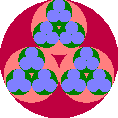
\includegraphics[width=2.0in]{3adicpic.pdf}
\caption*{Figure for Exercise \ref{ex:3adicpic}.}
\end{figure}

Here are some examples of elements of $\Z_5$: 
\small\begin{align*}  (101\bmod{5}, 101\bmod{5^2}, 101\bmod{5^3}, \dots) &=  (1\bmod{5}, 1\bmod{5^2}, 101\bmod{5^3}, \dots),  \\
(-1\bmod{5}, -1\bmod{5^2}, -1\bmod{5^3}, \dots) &= (4\bmod{5}, 24\bmod{5^2}, 124\bmod{5^3}, \dots), \\
(4\bmod{5}, 34\bmod{5^2}, 334\bmod{5^3}, \dots) &= (4\bmod{5}, 9\bmod{5^2}, 84\bmod{5^3}, \dots).
\end{align*}
Take a moment to convince yourself that this last example satisfies our compatibility condition!

\normalsize

\begin{prob}\label{prob:52} $\Z_p$ is a subring of $\prod_{k=1}^{\infty}\Z/p^k$.
\end{prob}

\begin{prob}\label{prob:53} $\Z_p$ is an integral domain.
\end{prob}

\begin{prob}\label{ex:embedding0}\label{prob:54} $\Z_p$ has characteristic $0$. (Thus, $\Z$ sits canonically inside $\Z_p$.)\\
Which elements of $\Q$ can be said to belong to $\Z_p$? Is our third example of a $5$-adic integer an element of $\Q$? (Assume the $n$th component is $3\dots 34\bmod{5^n}$, where $3$ is repeated $n-1$ times.)
\end{prob}

\begin{prob}\label{prob:55} $u = (a_1\bmod{p}, a_2\bmod{p^2}, \dots) \in \Z_p$ is a unit $\Longleftrightarrow$ $p\nmid a_1$ (in $\Z$) $\Longleftrightarrow$ $p\nmid u$ (in $\Z_p$).
\end{prob}


\begin{prob}\label{prob:56} Every nonzero element of $\Z_p$ admits a unique expression in the form $p^v u$, where $v$ is a nonnegative integer and $u$ is a unit in $\Z_p$.
\end{prob}

\begin{prob}\label{prob:57} $\Z_p$ is a principal ideal domain with $p\Z_p$ its only nonzero prime ideal.
\end{prob}

\begin{prob}\label{prob:58}\label{prob:justice} The canonical inclusion $\Z\hookrightarrow \Z_p$ induces an isomorphism $\Z/p^n \cong \Z_p/p^n\Z_p$, for every positive integer $n$.\end{prob}

\begin{prob}\label{prob:59} The definition of $\Z_p$ makes sense without requiring $p$ to be prime. However, considering $\Z_g$ for composite $g$ does not give anything essentially new. In fact: $\Z_{g}\cong \prod_{p\mid g} \Z_p$ for each integer $g>1$. (For instance, $\Z_{10} \cong \Z_2\times \Z_5$.)\index{$\Z_g$, ring of $g$-adic integers!decomposition as $\prod_{p\mid g}\Z_p$}
\end{prob}


\begin{prob}\label{ex:3adicpic}\label{prob:60} What does the picture on this page --- created by \TeX~StackExchange user \texttt{
Qrrbrbirlbel}\footnote{\url{https://tex.stackexchange.com/a/695157}} --- have to do with $\Z_3$?
\end{prob}


\begin{prob}[Steuding]\label{ex:dali} Repeat the last exercise for Salvador Dali's painting \emph{La Cara de la Guerra}.\index{La Cara de la Guerra}
\end{prob}

\begin{prob}[$\Z_p$ is uncountable]\label{prob:61} There is no map from $\Z^{+}$ \underline{onto} $\Z_p$.
\end{prob}

\vspace{-0.1in}
\section*{Well, Color Me Impressed!}
\begin{prob}[Thomas, Monsky]\label{prob:62} Consider the following $3$-coloring of the rational plane $\Q^{2}$: $(x,y)$ is \textsf{red} if $|x|_2 < 1, |y|_2 < 1$, \textsf{blue} if $|x|_2 \ge 1$, $|x|_2 \ge |y|_2$, and \textsf{green} if $|y|
_2 \ge 1$, $|y|_2 > |x|_2$. Show that any trio of differently colored points forms a triangle $\Delta$ with $|\mathrm{Area}(\Delta)|_2 > 1$.

{\scriptsize This observation plays a key role in the proof of \textsf{Monsky's Theorem}\index{Monsky's theorem}: \emph{It is impossible to dissect a square into an odd number of triangles all of which have the same area.}}
\end{prob}
